Модуль позволяет балансировать во время зарядки от 2 до 8 ячеек. 
Контроллер собирает данные о напряжения и температурах(через терморезисторы прикреплённые к аккумуляторам).
Плата оснащена CAN модулем.
Принципиальная схема, трассировка и файлы для производства были созданы в программе KiCad.

\begin{figure}[h!]
	\centering
	\begin{minipage}{0.45\linewidth}
		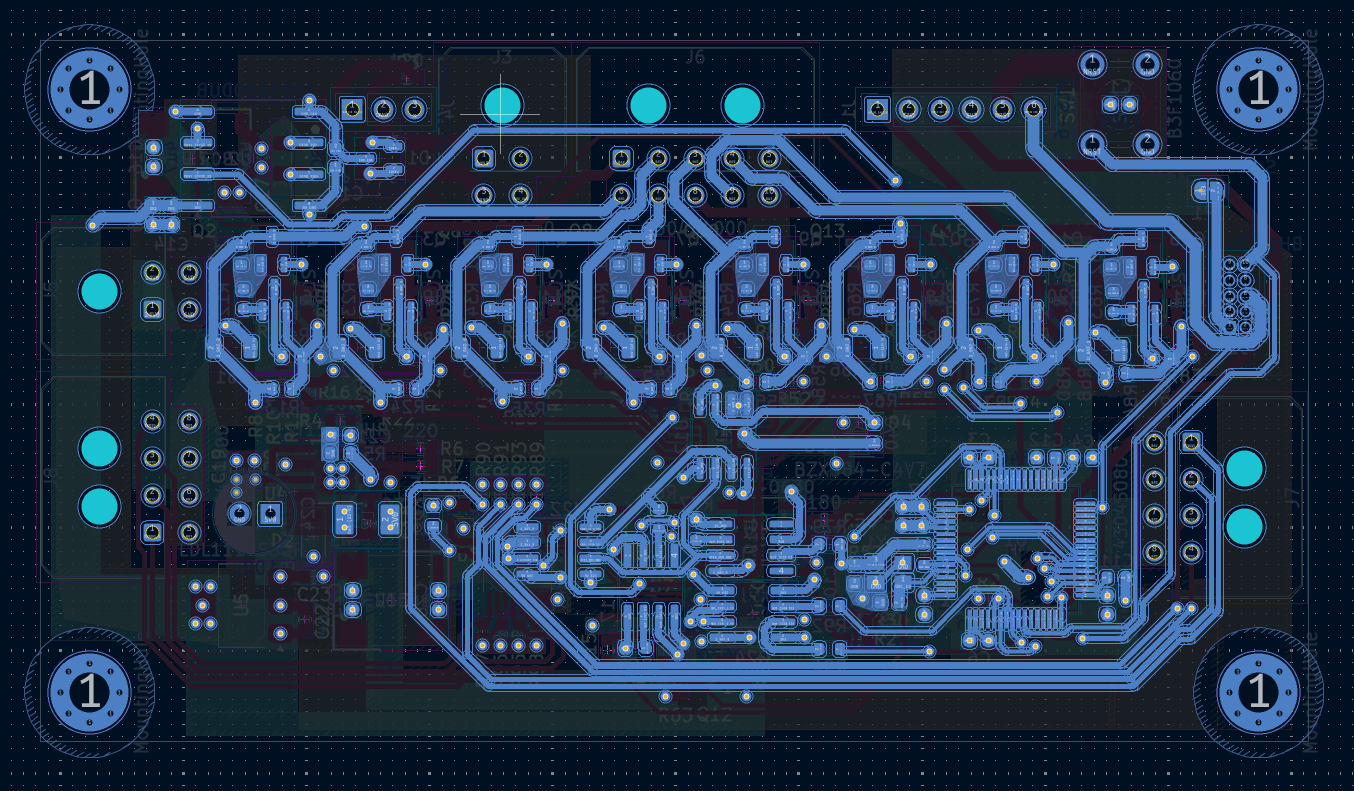
\includegraphics[width=\linewidth]{img/fb_traccing.png}
		\subcaption{Демонстрация трассировки платы}
	\end{minipage}
	\begin{minipage}{0.45\linewidth}
	    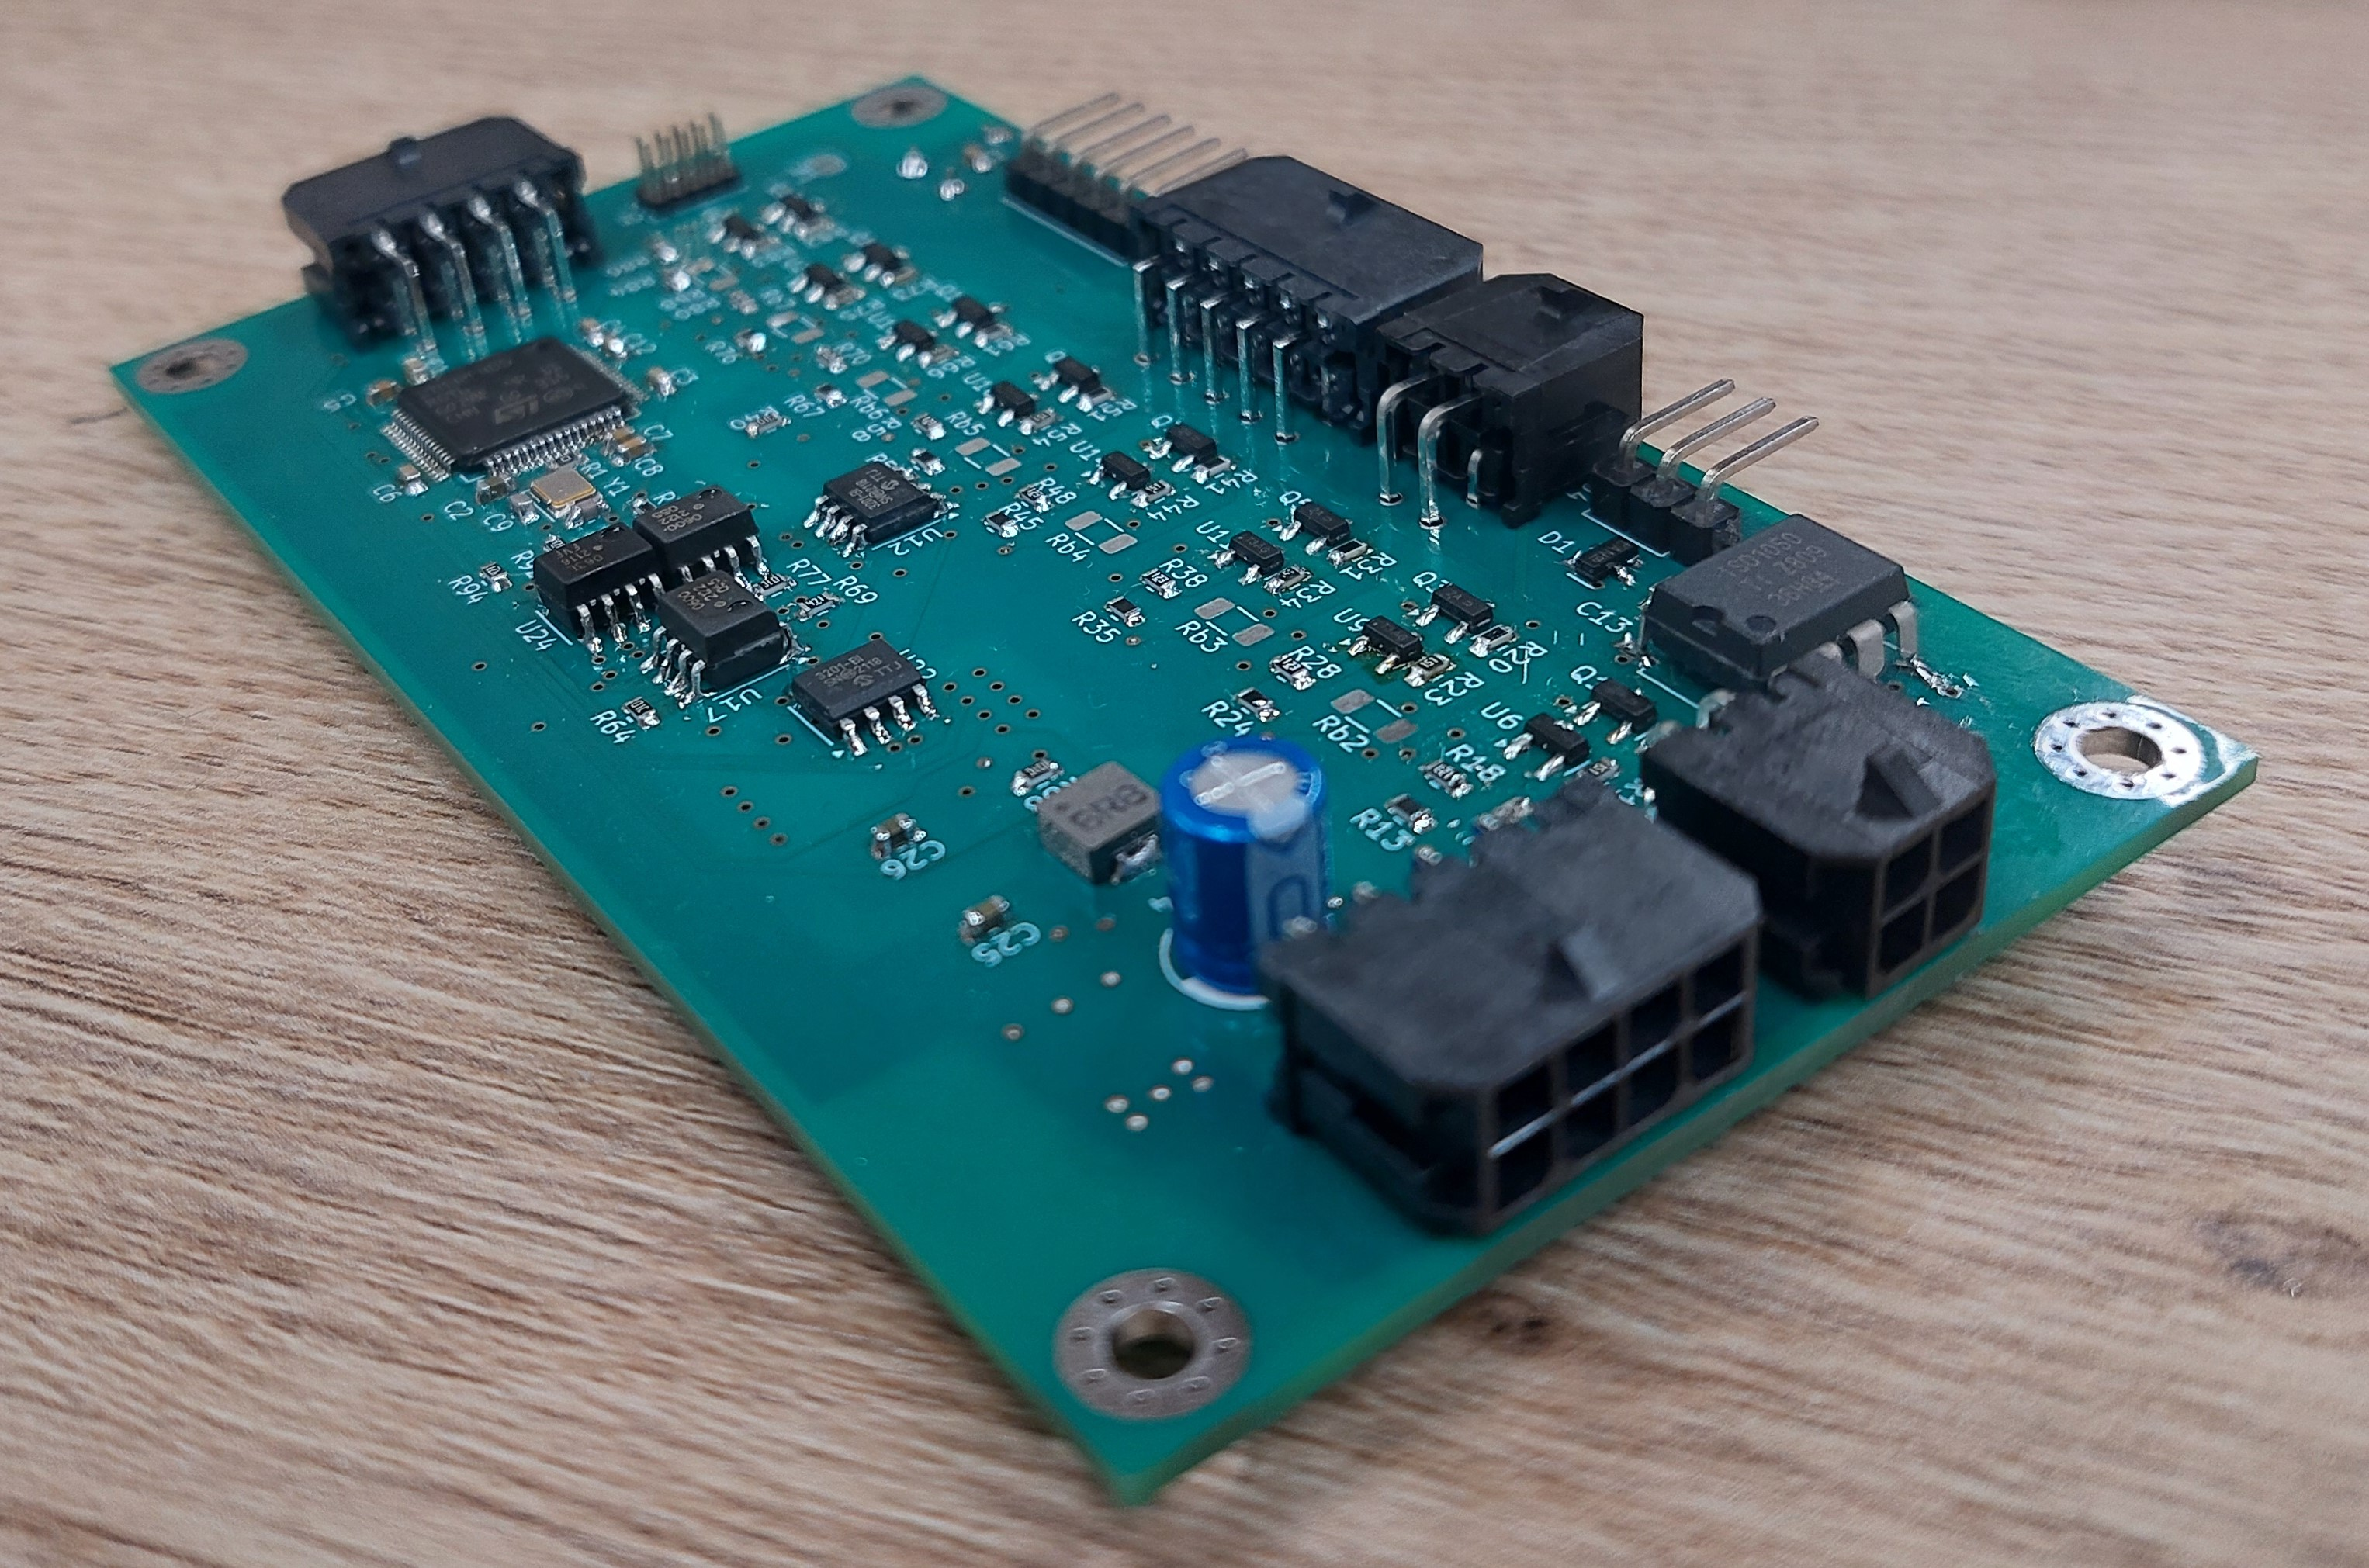
\includegraphics[width=\linewidth]{img/fabrication_ready.jpg}
	    \subcaption{Плата после сборки}
        \label{fig:fabrication_ready}
    \end{minipage} \\	
    \caption{Фотографии с производства}
    \label{fig:fabrication_traccing}
\end{figure} 

